\documentclass[12pt]{article}
\usepackage{a4wide}
\usepackage{color, amssymb}
\usepackage[margin=1in]{geometry}
\usepackage[document]{ragged2e}
\usepackage[table]{xcolor}
\usepackage{multirow}
\usepackage{hyperref}
\hypersetup{
    colorlinks=true,
    linkcolor=blue,     
    urlcolor=blue,
    pdfpagemode=FullScreen,
    }
\usepackage[braket, qm]{qcircuit}
\setlength{\arrayrulewidth}{0.5mm}
\setlength{\tabcolsep}{16pt}
\renewcommand{\arraystretch}{1.9}
\usepackage[english]{babel}
\usepackage{mathtools}
\usepackage{amsmath}
\usepackage{ragged2e}
\renewcommand{\baselinestretch}{1.5}
\input{epsf}
\usepackage{float}
\usepackage{graphicx}
\usepackage{braket}
\usepackage{caption}
\usepackage{subcaption}
\usepackage{algorithm}
\usepackage[noend]{algpseudocode}
\usepackage[math]{cellspace}
\usepackage[braket]{qcircuit}

\cellspacetoplimit = 3pt
\cellspacebottomlimit = 3pt

\begin{document}
\noindent\rule{\textwidth}{2pt}
\begin{center}
\large
{\bf Reinforcement Learning and Dynamic Optimization}\\ 
\normalsize
{\bf Kalamarakis Theodoros:} 2018030022\\
{\bf Toganidis Nikos:} 2018030085\\
{\it September 7, 2023}\\
\end{center}
\rule{\textwidth}{.5pt}
\noindent


\justifying

   \begin{center}
       \vspace*{0.5cm}
           
       \LARGE
       \textbf{Network Friendly Recommendations Project part II}
         
   \end{center}

\section*{{\bf Introduction}}
In the initial phase of our project, we designed a network-fiendly recommendation system. Its core objective was to identify the optimal batch of video recommendations 
for each video a user views. This recommendation batch should ensure two things: first, every recommended video should be closely related to the one the user has just watched,
 and second, it should be cached. To address this challenge, we employed a tabular Q-Learning algorithm. While this method proved effective for a limited set of videos,
  its efficiency decreased significantly as the number of videos increased. The root of this inefficiency lies in the vast action space. This space is directly proportional to the combinations 
  of videos in the recommendation batch, resulting in an action space size of ${K \choose N}=O(K^N)$, where $K$ represents the total videos in the library and $N$ denotes the videos in the recommendation batch. 
  In this phase of the project, we have change our approach to better address the issue. We integrated the {\bf SlateQ} algorithm by Google, which manages to completely bypass the action space altogether, 
  effectively reducing the complexity to $O(K)$.
\section*{{\bf Environment description and parameter selection}}
\begin{itemize}
    \item {\bf States}: As in the first phase,the implemented MDP environment represents a content recommendation system with a content
    catalogue consisting of K items. Each item corresponds to a state, where state $i$ represents the user
    watching video $i$. Therefore, there are K states in total.
    \item {\bf Action} The actions are the recommendation batch of $N$ videos. However the slateQ algorithm completely avoids any referance to the action set, so in practice, the action has no use
    \item {\bf Cost} The costs associated with watching a video depend on whether it is cached or not. If a video is
    cached, its cost is 0. If it is not cached, the cost is 1.
    \item {\bf Rewards} The rewards in this environment are defined as $reward_i = 1 - 2\cdot cost_i$. Therefore, if a video is cached,
    the reward is 1, and if it is not cached, the reward is -1. In the previous phase we used the $reward_i = 1 - cost_i$, but we observed faster convergence with the updated version
    \item   The parameter $\gamma$ (discount factor), $\epsilon$ (exproration-exploitation trade off parameter for $\epsilon$-greedy) and $\alpha$ (learning rate) are the same as in part 1. Specificaly:
    \begin{itemize}
        \item $\gamma = 1-q$
        \item $\epsilon = \frac{1}{t^{1/3}}(\#num \;of \;states\cdot \log t )^{1/3} $  where t is the number of episodes
        \item $\alpha = 0.01$
    \end{itemize}
   
\end{itemize}
 
\section*{{\bf SlateQ}}
In the tabular Q-Learning algorithm, the optimal Q-value can be approximated using the following update rule
$$Q^t(s,A) = Q^{t-1}(s,A) + \alpha\left(R(s,A,s') + \max_{A'}\left(\gamma Q^{t-1}(s',A')\right) - Q^{t-1}(s,A)\right)$$
The dimensions of matrix $Q(s,A)$ is $num\; of \; state\times num\;of\;actions = K\times {K \choose N}$, therefore it requires a considerable amount of time to be filled as $K$ and $N$ increase. 
To avoid the exhaustive exploration of the entire action space, SlateQ introduces an alternative function the $\bar{Q}(s,i)$. 
This function quantifies the value of being in state $s$ and choosing item $i$ from the recommendation batch, corresponding to action $A$, meaning that, $i\in A$.
$\bar{Q}(s,i)$ can be updated using the same target as $Q(s,A)$. Thus:
\begin{align*}
    \bar{Q}^t(s,i) = \bar{Q}^{t-1}(s,i) + \alpha\left(R(s,A,s') + \max_{A'}\left(\gamma Q^{t-1}(s',A')\right) - \bar{Q}^{t-1}(s,i)\right) \tag{1}
\end{align*}
    In our environment we consider if $s' = i$ with probability 1 if $i$ is selected by the user, therefore $R(s,A,s') = R(s,i)$. Furthermore it can be proven (see the cited paper) that 
$$Q(s,A) = \sum_{i\in A}P(i|s,A)\bar{Q}(s,i)$$
So equation $(1)$ becomes:
\begin{align*}
    \bar{Q}^t(s,i) = \bar{Q}^{t-1}(s,i) + \alpha\left(R(s,i) + \max_{A'}\left(\gamma \sum_{j\in A'}P^{t-1}(j|i,A')\bar{Q}^{t-1}(i,j)\right) - \bar{Q}^{t-1}(s,i)\right) 
\end{align*}

Having established our update rule, we now address the maximization problem:
$$\max_{A}\sum_{i\in A}P(i|s,A)\bar{Q}(s,i)$$
Given that the likelihood of selecting item $i$ from $N$ recommendations is $\frac{1}{N}$, we can express this as
$$\max_{A}\sum_{i\in A}P(i|s,A)\bar{Q}(s,i) = \max_{A}\sum_{i\in A}\frac{1}{N}\bar{Q}(s,i) $$
if we define the vector $\bf x$ such that $x_i= 1$ if $i\in A$ and $x_i = 0$
if $i \notin A$ for $i \in \{1,...,K\}$, we coclude to the maximaization problem

\begin{equation}
\begin{aligned}
& \underset{\bf x}{\text{maximize}}
& & \sum_i x_i\frac{1}{N}\bar{Q}(s,i) \\
& \text{subject to}
& &x_i \in \{0,1\} \\
& & & \sum_{i} x_i = N,
\end{aligned}
\end{equation}To transform this into a linear optimization problem, we can relax the first constraint, resulting in: 
\begin{equation}
    \begin{aligned}
    & \underset{\bf x}{\text{maximize}}
    & & \sum_i x_i\frac{1}{N}\bar{Q}(s,i) \\
    & \text{subject to}
    & &x_i \in [0,1] \\
    & & & \sum_{i} x_i = N,
    \end{aligned}
    \end{equation}
After the maximization process, the values of $x_i$ will converge to binary values  $\{0,1\}$

\section*{{\bf Experimental Evaluation}}

To evaluate the effectiveness of the algorithm, we employ a simulation function. This function 
takes the policy derived from SlateQ and uses it to run multiple episodes in the environment, 
ultimately calculating an average cost per session.In the first phase of the project, 
we developed a formula that calculates the minimum average cost of a session, $E(S)$, 
for a fixed number of cached items $C=0.2K$, given the parameters $\alpha$ and $q$. Essentially, 
this formula indicates the optimal average cost to which our algorithm should converge as $K \rightarrow \infty$. 
The formula is presented below, and its proof can be found in the appendix.

\begin{align*}
    E[S] = 0.8 + 0.8(\frac{1}{q}-1)(1-\alpha) \tag{3}
\end{align*}
Now if we set $\alpha = 0.8$ and $q=0.2$ we get
\begin{align*}
    E[S] = 0.8 + 0.8(\frac{1}{0.2}-1)(1-0.8) = 1.44 
\end{align*}
Which means that, for those parameters, the optimal policy should yield an average cost of $1.44$. Below, 
we present the simulation results of the policies generated by both Q-Learning and SlateQ for $C=0.2K$, $\alpha = o.8$, $q= 0.2$ and $u_{min} = 0.2$ We can compare them in 
terms of average cost over $K$ and elapsed time over $K$.$C=0.2K$, $\alpha = o.8$, $q= 0.2$, $u_min = 0.2$

\begin{figure}[H] % h = here, t = top, b = bottom, p = separate figure page
    \centering
    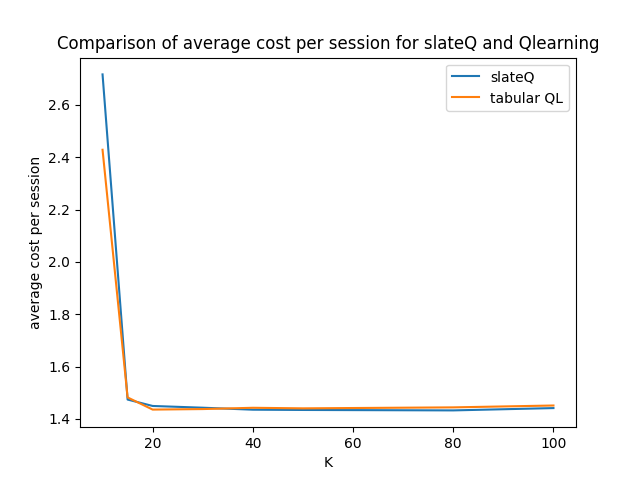
\includegraphics[width=0.49\linewidth]{Figure_1.png}
    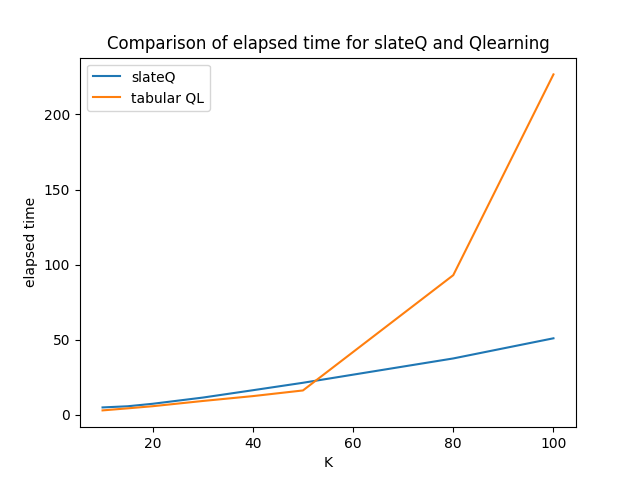
\includegraphics[width=0.49\linewidth]{Figure_2.png}
    \caption{Comparing average cost per session (left) and elapsed time (right) over $K$ of SlateQ and Q-Learning for parameters$N=2$ $C=0.2K$, $\alpha = o.8$, $q= 0.2$, $u_{min} = 0.2$.}
    %\label{fig:my_label}
\end{figure}

In the figure above, we note that the average cost per session for SlateQ not only aligns with that of Q-Learning (which we use as a benchmark for correct operation), but it also converges to the desired cost of $1.44$. 
This suggests that SlateQ effectively reaches one of the optimal policies. Regarding the elapsed time, we notice that SlateQ exhibits a roughly 
linear increase with respect to $K$, in contrast to Q-Learning, which appears to escalate exponentially. Hence, we now shift our focus solely to SlateQ and aim to determine its "breaking point."
 We set $N=10$ and increment $K$ up to 1000! Below are the results
 \begin{figure}[H] % h = here, t = top, b = bottom, p = separate figure page
    \centering
    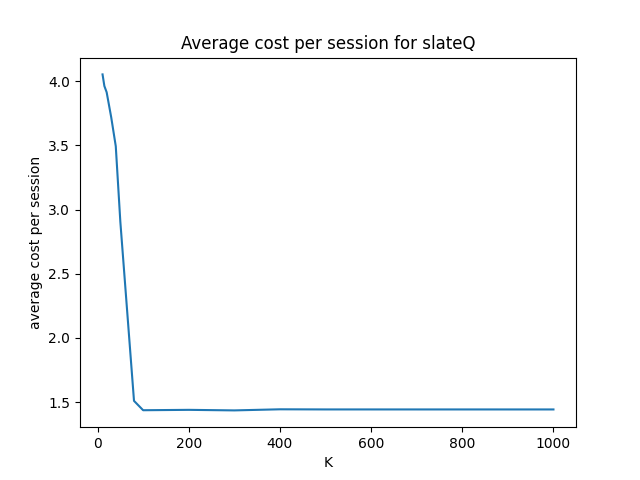
\includegraphics[width=0.49\linewidth]{Figure_3.png}
    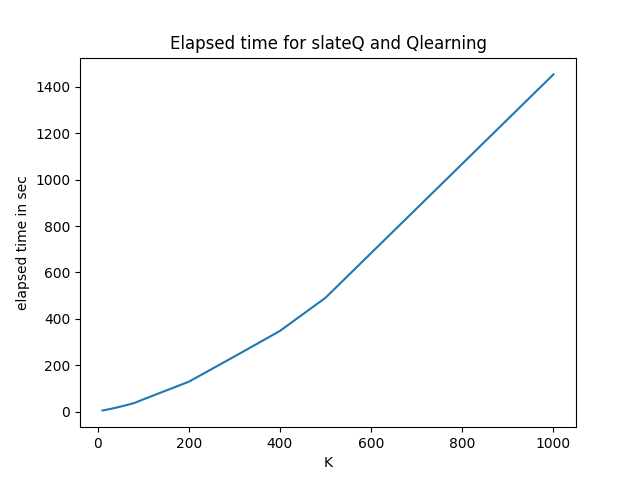
\includegraphics[width=0.49\linewidth]{Figure_4.png}
    \caption{Average cost per session (left) and elapsed time (right) over $K$ of SlateQ for parameters $N=10$, $C=0.2K$, $\alpha = o.8$, $q= 0.2$, $u_{min} = 0.2$.}
    %\label{fig:my_label}
\end{figure}
We note that even with such a large library, the algorithm consistently identifies the optimal policy, as the average cost per session remains at the optimal $1.44$. 
Additionally, the elapsed time continues its, sort of, linear increase. 
These observations are undeniable indications that the algorithm operates as anticipated
\section*{{\bf Additional Plots}}
below we present  escalation of average cost per session and elapsed time w.r.t $N$
\begin{figure}[H] % h = here, t = top, b = bottom, p = separate figure page
    \centering
    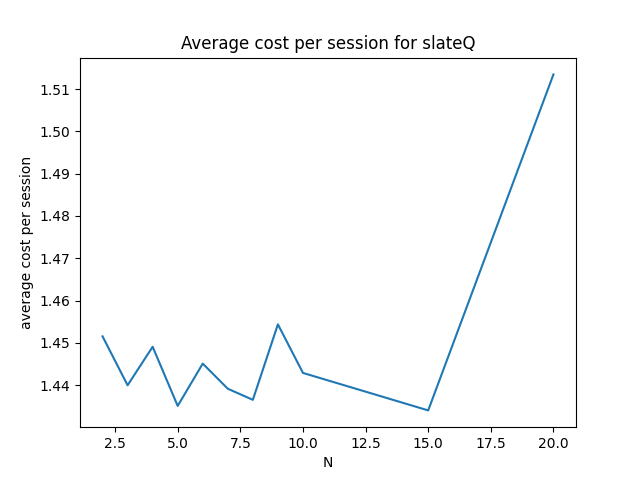
\includegraphics[width=0.49\linewidth]{Figure_5.png}
    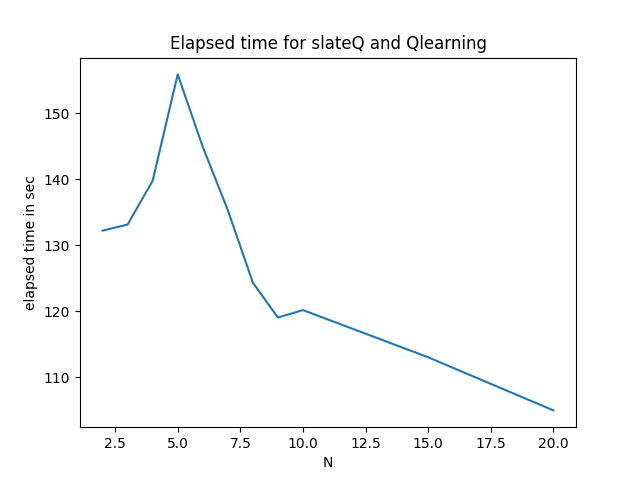
\includegraphics[width=0.49\linewidth]{Figure_6.png}
    \caption{Average cost per session (left) and elapsed time (right) over $N$ of SlateQ for parameters $K=200$, $C=0.2K$, $\alpha = o.8$, $q= 0.2$, $u_{min} = 0.2$.}
    %\label{fig:my_label}
\end{figure}
We observe that throughout the experiment, the average cost consistently remains at $1.44$, except when N=20N=20, at which point the average cost experiences a slight increase.
Finally we present the escalation of the average cost per session w.r.t $\alpha$, $q$, $u_{min}$

\begin{figure}[H] % h = here, t = top, b = bottom, p = separate figure page
    \centering
    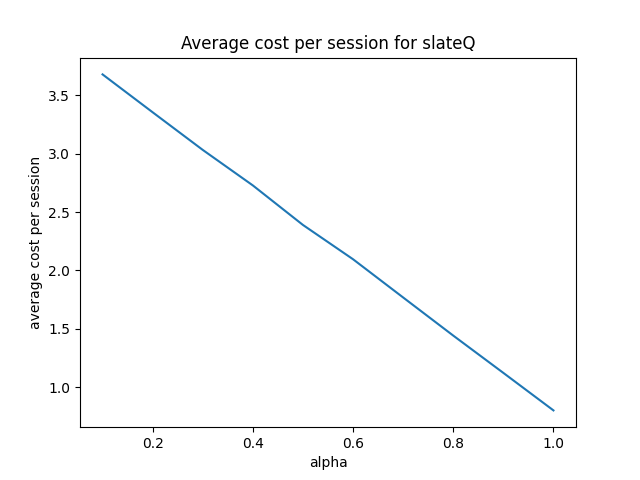
\includegraphics[width=0.49\linewidth]{Figure_7.png}
    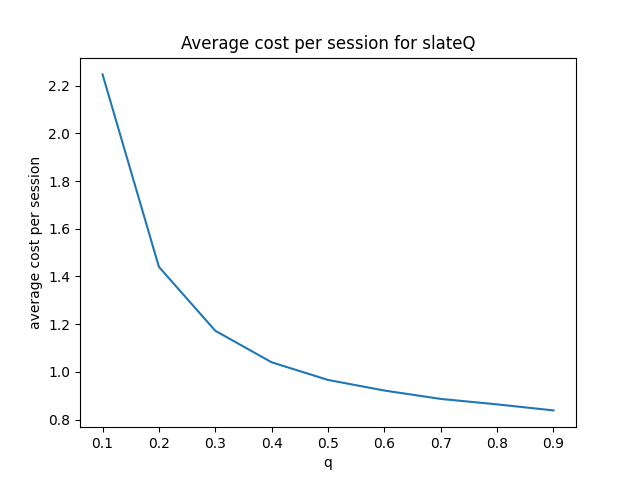
\includegraphics[width=0.49\linewidth]{Figure_8.png}\\
    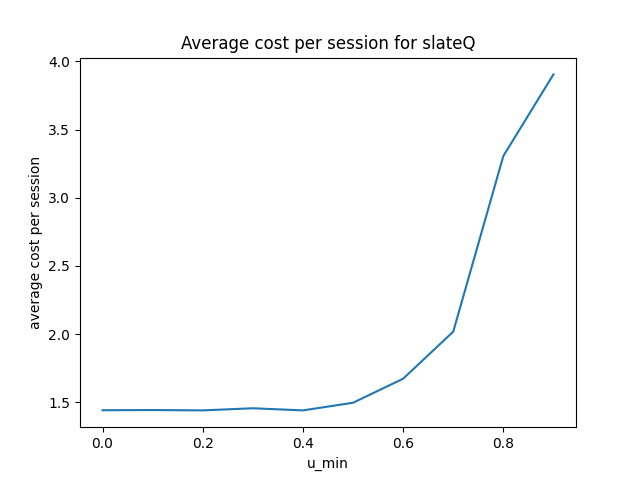
\includegraphics[width=0.49\linewidth]{Figure_9.png}
    \caption{Average cost per session over $alpha$ (top left), $q$ (top right), $u_{min}$ (bottom) of SlateQ for parameters $K=100$, $C=0.2K$ .}
    %\label{fig:my_label}
\end{figure}
\section*{Referances}

\url{https://arxiv.org/pdf/1905.12767.pdf}\\
\section*{{\bf Appendix}}
\subsection*{Proof of formula (3)}
Initially, we need to calculate the average cost of watching a video given the parameter $\alpha$. Let $X \in \{0, 1\}$ be the cost of a video. Then we have:
\begin{equation}
E[X] = 0 \times P(C) + 1 \times P(U) = P(U)
\end{equation}
where $P(C)$ is the probability of the video being cached and $P(U)$ is the probability of the video being uncached.
\begin{equation}
P(U) = P(U|A)P(A) + P(U|\bar{A})P(\bar{A})
\end{equation}
Here, $A$ denotes the event of choosing a video from the recommendation batch, so $P(A) = \alpha$. Since we are interested only in large $K$, we can assume that no item in the recommendations batch is uncached, making the probability of choosing an uncached video from the recommendations zero ($P(U|A) = 0$). On the other hand, choosing an uncached video out of all videos has a probability of $0.8$.
\begin{equation}
P(U) = P(U|A)P(A) + P(U|\bar{A})P(\bar{A}) = 0.8(1 - \alpha)
\end{equation}
To calculate the average cost of a session, it might seem logical to multiply the average number of videos during a session with the average cost of a video ($E[X]$). However, due to the initial state being chosen randomly with an average cost of $0.8$, we need to consider it separately. Let the average number of videos in a session be $E[n] = \frac{1}{q}$, then the average cost of the session can be calculated as:
\begin{equation}
E[S] = 0.8 + (E[n] - 1)E[X] = 0.8 + 0.8(\frac{1}{q}-1)(1 - \alpha)
\end{equation}
Note that the constant $0.8$ corresponds to $1 - \frac{C}{K}$ for $C = 0.2K$. Therefore, the general formula for any value of $C$ would be:
\begin{equation}
E[S] = \left(1 - \frac{C}{K}\right) + \left(1 - \frac{C}{K}\right)\left(\frac{1}{q}-1\right)\left(1 - \alpha\right)
\end{equation}
Plotting $E[S]$ against $C$ will reveal a linear decreasing relationship.
\end{document}